\documentclass[letterpaper]{article}

\usepackage{ifthen}
\usepackage{xparse}
\usepackage{enumitem}
\usepackage[utf8]{inputenc}
\usepackage{amsmath}
\usepackage{amssymb}
\usepackage{stmaryrd}
\usepackage{amsthm}
\usepackage{mathtools}
\usepackage{proof}
\usepackage{colonequals}
\usepackage{comment}
\usepackage{textcomp}
\usepackage[us]{optional}
\usepackage{color}
\usepackage{url}
\usepackage{verbatim}
\usepackage{graphics}
\usepackage{mathpartir}
\usepackage{tikz}
\usepackage{todonotes}

% these two are used to create the wavy division sign
\usepackage{stackengine}
\usepackage{scalerel}

\usepackage{hyperref}
\usepackage[nameinlink, capitalise]{cleveref}

\usepackage{array}


%% Beamer defines a range of its own theorems
\ifx\beamer\undefined

\theoremstyle{plain}
\newtheorem{theorem}{Theorem}[section]
\newtheorem{lemma}[theorem]{Lemma}
\newtheorem{corollary}[theorem]{Corollary}

\theoremstyle{definition}
\newtheorem*{remark}{Remark}
\newtheorem*{notation}{Notation}
\newtheorem{definition}{Definition}
\newtheorem{conjecture}{Conjecture}
\newtheorem{example}{Example}

\else 
  %% Intentionally left blank
\fi

\makeatletter
\newcommand\xlabel[2][]{\phantomsection\def\@currentlabelname{#1}\label{#2}}
\makeatother

\newenvironment{rules}[1][{}]{\begin{mathpar}}{\end{mathpar}}

%% This puts the name on the top
\NewDocumentCommand{\defrule}{o o m m}{
  \inferrule*[lab=\IfNoValueTF{#1}{}{\textsc{[#1]}}]
  { #3 }
  { #4 }
  \IfNoValueTF{#2}{}{\xlabel[#1]{\ifdefined\InApx{apx:}\else\fi#2}}
}


\NewDocumentCommand{\ruleref}{m}{{[\textsc{\nameref{#1}}]}}


\usepackage[abt]{pfpl-syntax}
\usepackage{pfpl-judgments}

%% \xMapsto command
% \usepackage{mathtools}
\usepackage{stmaryrd}

\makeatletter
\newcommand{\xMapsto}[2][]{\ext@arrow 0599{\Mapstofill@}{#1}{#2}}
\def\Mapstofill@{\arrowfill@{\Mapstochar\Relbar}\Relbar\Rightarrow}
\makeatother

%% Instructor-only remarks. These remarks requires the benefit of the hind sight to understand
%% (or foreshadowing) future content so it doesn't make sense to put it in the file
%% Define \isstudentcopy to generate the student version
\definecolor{iremarkcolor}{rgb}{0.0, 0.0, 0.5}
\NewDocumentEnvironment{iremark}{ +b }
{ \ifthenelse{\isundefined{\isstudentcopy}}{
    \begingroup
    \color{iremarkcolor}
    \begin{remark}
    #1
    \end{remark}
    \endgroup
  }{
  }
}{ }

\newcommand{\inlremark}[1]{\ifthenelse{\isundefined{\isstudentcopy}}{\begingroup\color{iremarkcolor}(#1)\endgroup}{}}
\newcommand{\PFPL}{\textbf{\textsf{PFPL}}}
\makeatletter

\NewDocumentCommand{\fstEx}{s O{\tau_1} O{\tau_2} m}{\IfBooleanTF{#1}{\projEx*<1>[#2][#3]{#4}}{\projEx<1>[#2][#3]{#4}}}
\NewDocumentCommand{\sndEx}{s O{\tau_1} O{\tau_2} m}{\IfBooleanTF{#1}{\projEx*<2>[#2][#3]{#4}}{\projEx<2>[#2][#3]{#4}}}

\NewDocumentCommand{\hatM}{}{\hat{M}}

\NewDocumentCommand{\Iff}{}{\,\mathrm{iff}\,}
\NewDocumentCommand{\limp}{}{\supset}

\NewDocumentCommand{\HT}{O{A}}{\mathsf{HT}_{#1}}


\makeatother



\usepackage{tikz}
\usetikzlibrary{automata,positioning}

\newcommand{\gmhat}[1]{\ensuremath{\widehat{\gamma}(#1)}}

\title{15-791 ATPL \\ Week 2 Notes}
\author{Hemant Gouni and Josh Grosso}
\date{\today}

\begin{document}

\maketitle

\section{Natural Numbers and Co-Natural Numbers}

\subsection{Co-Natural Numbers}

We extend our language from the previous lecture with a simple coinductive
type, in particular conatural numbers. The grammar is given by

$$
A \coloncolonequals \cdots \mid \conatTy
$$
$$
M \coloncolonequals \cdots \mid \outEx*{M} \mid \genEx*{M}{x}{N}
$$

\noindent
The statics is given in a standard way:

\begin{mathpar}
% TODO: ensure I, E are correct here
\defrule[T-Conat-I][sta:gen]
    {\Gamma \entails{\isOfTp{M}{A}} \\ \Gamma, \isOfTp{x}{A} \entails{\isOfTp{N}{\sumTy*{\unitTy*}{A}}}}
    {\Gamma \entails{\isOfTp{\genEx*{M}{x}{N}}{\conatTy}}}

\defrule[T-Conat-E][sta:out]
    {\Gamma \entails{\isOfTp{M}{\conatTy}}}
    {\Gamma \entails{\isOfTp{\outEx*{M}}{\sumTy*{\unitTy*}{\conatTy}}}}
\end{mathpar}

\noindent
Along with a call-by-name transition system for the dynamics:

\begin{mathpar}
\defrule[V-Gen][dyn:gen-val]
    {}
    {\isVal{\genEx*{M}{x}{N}}}

\defrule[D-Pred-C][dyn:pred-c]
    {M \stepsTo{} M'}
    {\outEx*{M} \stepsTo{} \outEx*{M'}}

\defrule[D-Pred-1][dyn:pred-1]
    {}
    {\outEx*{\genEx*{M}{x}{N}} \mapsto \xcaseEx*{\Sub{M}{x}{N}}{\_}{\injEx*<1>{\unitEx*}}{y}{\injEx*<2>{\genEx*{y}{x}{N}}}}
\end{mathpar}

\subsection{Co-Naturals as State Machines}

\noindent
The semantics of $\genEx*{M}{x}{N}$ bears explanation. Conatural numbers can be
understood in terms of \textit{state machines}. Describing $\genEx*{M}{x}{N}$
in the language of state machines:

\begin{enumerate}
    \item $M$ is the prior state
    \item $N$ is the state transformer, determining the next state
    \item $\outEx*{}$ induces a transition to the next state
\end{enumerate}

\begin{figure}[h]
\begin{center}
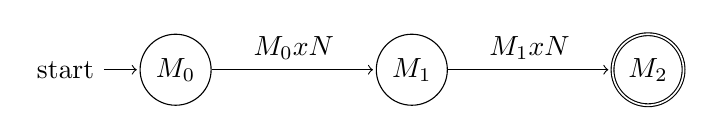
\begin{tikzpicture}[shorten >=1pt,node distance=3cm,on grid,auto]
    \node[state,initial] (M_0) {$M_0$};
    \node[state] (M_1) [right=of M_0] {$M_1$};
    \node[state,accepting](M_2) [right=of M_1] {$M_2$};
      \path[->]
      (M_0) edge node {$\Sub{M_0}{x}{N}$} (M_1)
      (M_1) edge node {$\Sub{M_1}{x}{N}$} (M_2);
\end{tikzpicture}
\end{center}
\caption{A simple state machine}
\label{fig:state-machine-1}
\end{figure}

For a concrete example, consider the machine in \ref{fig:state-machine-1}.
$M_0$ is the initial state. We can think about invoking
$\outEx*{\genEx*{M_0}{x}{N}}$ to get to the next state $M_1$. $M_1$ is
calculated by evaluating $\Sub{M_0}{x}{N}$. In this example $M_1$ is not a
(doubly-circled) end state--- in other words, it's not of unit type--- so by
\ruleref{dyn:pred-1} we get a new value $\genEx*{M_1}{x}{N}$. Observe that in
order to transition to the next state, we must invoke
$\outEx*{\genEx*{M_1}{x}{N}}$ once more. $\genEx*{M_1}{x}{N}$ by itself does
not compute further.

The next transition operates similarly, with the exception of resulting in a
unit value. In this case, we can no longer induce any further transitions
because we're not left with a \texttt{gen} form.

\begin{figure}[h]
\begin{center}
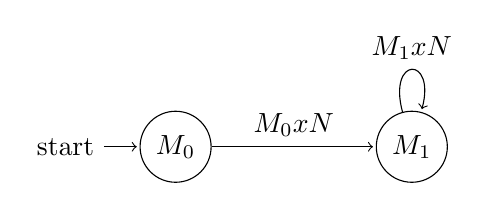
\begin{tikzpicture}[shorten >=1pt,node distance=3cm,on grid,auto]
    \node[state,initial] (M_0) {$M_0$};
    \node[state] (M_1) [right=of M_0] {$M_1$};
      \path[->]
      (M_0) edge node {$\Sub{M_0}{x}{N}$} (M_1)
      (M_1) edge [loop above] node {$\Sub{M_1}{x}{N}$} ();
\end{tikzpicture}
\end{center}
\caption{A state machine without an end state}
\label{fig:state-machine-2}
\end{figure}

It is also worth noting that, as shown in \ref{fig:state-machine-2}, the state
machine represented by a \texttt{conat} \textit{need not have an end state}. In
this instance, $\outEx*{\genEx*{M_1}{x}{N}}$ always evaluates to
$\genEx*{M_1}{x}{N}$--- never to $\unitEx*$. This is not a problem for
termination because, again, a $\genEx*{M_1}{x}{N}$ is inert until `kicked' by
using \texttt{out} on it.

\subsection{Termination for Co-Natural Numbers}

We can proceed with the proof of hereditary termination for co-natural numbers.

\begin{definition}[Hereditary termination for $\conatTy$]
    Define $\HT[\conatTy](M)$ on closed terms $M$ of type $\conatTy$ such that
    one of the following holds:
    \begin{enumerate}
        \item $\outEx*{M} \evalsTo \injEx*<1>{\unitEx*}$.
        \item $\outEx*{M} \evalsTo \injEx*<2>{M'}$ and $\HT[\conatTy](M')$
    \end{enumerate}
\end{definition}

Another way to state this is that $\HT[\conatTy](M)$ is the \textit{weakest}
(or \textit{largest}, when viewed as a set) property $\mathcal{P}$ on closed
terms $\isOfTp{M}{\conatTy}$ such that if $\mathcal{P}(M)$, then either:

\begin{enumerate}
    \item $\outEx*{M} \evalsTo \injEx*<1>{\unitEx*}$
    \item $\outEx*{M} \evalsTo \injEx*<2>{M'}$ and $\mathcal{P}(M')$
\end{enumerate}

% TODO: ask harrison about this
Observe this is dualized compared to the case for natural numbers, where having
the analogous properties implied $\mathcal{P}(M)$--- rather than
$\mathcal{P}(M)$ implying these properties. This mirrors the structure of
working (inductively) with natural numbers, versus working (coinductively) with
co-natural numbers.

In order to have a property of natural numbers, we must
evaluate it to know which case we're in, $\zeroEx*$ or $\succEx*{M'}$, and show
the property for it. In contrast, when we use $\outEx*$ on a $\conatTy$
satisfying the property and evaluate the resulting expression, we get something
back that satisfies the necessary properties, but we do not know precisely
which case does so.

% Intuitively, the requirement for $\HT[\conatTy](M)$ to be the $weakest$ such
% property arises from the fact that coinduction maps \textit{out}-- it
% represents a \textit{post fixed-point}. So we must find the \textit{greatest}
% post fixed-point (necessary property is consistency?) in order to reason about
% coinductive types.

\begin{theorem}[Fundamental Theorem]
If $\Gamma \entails{\isOfTp{M}{A}}$ then $\Gamma \gg M \in A$.
\end{theorem}

\begin{proof}
    Proceed by induction on a derivation of $\isOfTp{M}{A}$.
    \begin{enumerate}
        \item [\ruleref{sta:out}]
            Want to show if $\Gamma
            \entails{\isOfTp{\outEx*{M}}{\sumTy*{\unitTy*}{\conatTy}}}$ then
            $\Gamma \gg \outEx*{M} \in \sumTy*{\unitTy*}{\conatTy}$.
            We have by inversion that $\Gamma \entails{\isOfTp{M}{\conatTy}}$.
            Then by induction we know $\Gamma \gg M \in \conatTy$.
            We now want to show that $\HT[\sumTy*{\unitTy*}{\conatTy}](\gmhat{\outEx*{M}})$.
            We have to show that either $\gmhat{\outEx*{M}} \evalsTo
            \injEx*<1>{\unitEx*}$ or $\gmhat{\outEx*{M}} \evalsTo
            \injEx*<2>{M'}$ and $\HT[\conatTy](M')$.
            This is exactly the definition of $\HT[\conatTy](\gmhat{M})$, which
            we have by induction, so we're done.
        \item [\ruleref{sta:gen}]
            Want to show if $\Gamma
            \entails{\isOfTp{\genEx*{M}{x}{N}}{\conatTy}}$ then $\Gamma \gg
            \genEx*{M}{x}{N} \in \conatTy$.

            For convenience, define $G(-) \triangleq \genEx*{-}{x}{\gmhat{N}}$.
            Additionally, define $M_0 \triangleq \gmhat{M}$.
            We begin by reasoning about some $P$ which is consistent against
            $\HT[\conatTy]$.
            We'll show that this $P$ holds, and because $P$ implies
            $\HT[\conatTy]$ (by its consistency against the latter), we'll have
            the property. Let's list the properties we'd like out of $P$.
            For all $\isOfTp{M}{\conatTy}$:

            \begin{enumerate}
                \item if $P(M)$ then
                    $(\sumTy*{\unitTy*}{P})
                     \footnote{$(\sumTy*{\unitTy*}{P})(\outEx*{M})$ is
                     equivalent to evaluating and casing on $\outEx*{M}$, then
                     returning the left injection unmodified, or the right
                     injection with $P$ applied to it.}
                     (\outEx*{M})$
                     \label{itm:conat-p1}
                \item $P(G(M_0))$ \label{itm:conat-p2}
            \end{enumerate}

            % larger = weaker because it's easier to find an element of the set
            Any $P$ satisfying \ref{itm:conat-p1} is consistent against
            $\HT[\conatTy]$, therefore implying it, because $\HT[\conatTy]$ is
            defined to be the \textit{largest} such property-- so it contains
            $P$ (alternatively, it's the \textit{weakest} such property-- so
            it's implied by $P$). \ref{itm:conat-p2} will be important as the
            coinductive `base case', letting us get a foothold in the initial
            state so we can show the property coinductively for future states.
            Take the following to be the definition of $P$; we will show its
            consistency later:

            \begin{definition}[Definition of $P$]
                Define $P(M) \triangleq M \evalsTo G(M')$ for some $\HT[A](M')$.
            \end{definition}

            % To show that this satisfies consistency with $\HT[\conatTy]$, show
            % that if $P(X)$ then $(\sumTy*{\unitTy*}{P})(\outEx*{X})$.

            % \begin{proof}
            %     Assume $X \evalsTo G(M)$ with $\HT[A](M)$.
            %     Then in the first case:
            %     \begin{align*}
            %         \outEx*{X} \evalsTo&\, \outEx*{G(M)}\\
            %                    \evalsTo&\, (\sumTy*{\unitTy*}{G})(\Sub{M}{x}{N})\\
            %                    \evalsTo&\, \injEx*<1>{\unitEx*}
            %     \end{align*}
            %     Where consistency is immediate from the first case of
            %     $\HT[\conatTy]$. Or in the second case:
            %     \begin{align*}
            %         \outEx*{X} \evalsTo&\, \outEx*{G(M)}\\
            %                    \evalsTo&\, (\sumTy*{\unitTy*}{G})(\Sub{M}{x}{N})\\
            %                    \evalsTo&\, \injEx*<2>{G(M')}
            %     \end{align*}
            %     Where we have consistency if we have $\HT[A](M')$.
            % \end{proof}

            Observe that $P(G(M_0))$ holds, satisfying \ref{itm:conat-p2}.
            We have $\outEx*{G(M_0)} \evalsTo \Sub{M_0}{x}{N}$.
            By induction on the rule, $\HT[\sumTy*{\unitTy*}{A}](\Sub{M_0}{x}{\gmhat{M}})$.
            There are two cases here, drawn from hereditary termination at sum type:

            \begin{enumerate}
                \item $\Sub{M_0}{x}{\gmhat{N}} \evalsTo \injEx*<1>{\unitEx*}$
                \item $\Sub{M_0}{x}{\gmhat{N}} \evalsTo \injEx*<2>{M_1}$ with $\HT[A](M_1)$
            \end{enumerate}

            The first case is trivially consistent with $\HT[\conatTy]$.
            In the second case, we necessarily have $P(G(M_1))$ since
            $\HT[A](M_1)$ and because the form of the argument is as needed.
            Similarly for when we repeat the process on $P(G(M_1))$, we'll have
            $P(G(M_2))$, for the $M_2$ that arises out of the right injection
            as $M_1$ did.

            Observe that $P(G(M_i))$ holds for each element from the
            $\HT[A](M_i)$ obtained from the previous iteration.
            Then we can say $P$ is consistent against $\HT[\conatTy]$ due to
            its preservation of hereditary termination for each state which
            appears in the computation on a co-natural number, exactly as
            $\HT[\conatTy]$ is defined.
            So the complete chain of state transitions is consistent with
            $\HT[\conatTy]$.
            We have $P(G(M_0))$, where $M_0$ is the `start state', so we have
            $\HT[\conatTy](G(M_0))$ by virtue of it being the weakest such
            property.
            Recall that $M_0 \triangleq \gmhat{M}$, so we have
            $\HT[\conatTy](\gmhat{M})$, and therefore $\Gamma \gg
            \genEx*{M}{x}{N} \in \conatTy$ as desired.
            
            % \begin{figure}[h]
            % \begin{center}
            % \begin{tikzpicture}[shorten >=1pt,node distance=3cm,on grid,auto]
            %     \node[state,initial] (M_0) {$M_0$};
            %     \node[state] (M_1) [right=of M_0] {$M_1$};
            %     \node[state,accepting](M_2) [right=of M_1] {$M_2$};
            %       \path[->]
            %       (M_0) edge node {$\Sub{M_0}{x}{N}$} (M_1)
            %       (M_1) edge node {$\Sub{M_1}{x}{N}$} (M_2);
            % \end{tikzpicture}
            % \end{center}
            % \caption{A simple state machine}
            % \end{figure}
            
    \end{enumerate}
\end{proof}

\end{document}
